\documentclass[12pt]{article}
\usepackage{graphicx}
\usepackage{float}
\usepackage{amsmath}
\begin{document}
\title{Computer Science 145, Homework 5}
\date{March 6th, 2019}
\author{Michael Wu\\UID: 404751542}
\maketitle

\section*{Problem 1}

\paragraph{a)}

In the first iteration we obtain the following table.
\begin{center}
    \begin{tabular}{c|c}
        Item Set & Support \\
        \hline
        \(\{a\}\) & 6\\
        \(\{b\}\) & 8\\
        \(\{c\}\) & 6\\
        \(\{d\}\) & 4\\
        \(\{e\}\) & 2\\
        \(\{i\}\) & 1\\
        \(\{j\}\) & 1\\
        \(\{k\}\) & 1
    \end{tabular}
\end{center}
We can ignore \(\{i\}\), \(\{j\}\), and \(\{k\}\) since they are not frequent. Then we have the following length
two candidates and supports.
\begin{center}
    \begin{tabular}{c|c}
        Item Set & Support \\
        \hline
        \(\{a,b\}\) & 4\\
        \(\{a,c\}\) & 4\\
        \(\{a,d\}\) & 2\\
        \(\{a,e\}\) & 2\\
        \(\{b,c\}\) & 4\\
        \(\{b,d\}\) & 4\\
        \(\{b,e\}\) & 2\\
        \(\{c,d\}\) & 1\\
        \(\{c,e\}\) & 1\\
        \(\{d,e\}\) & 0\\
    \end{tabular}
\end{center}
We can ignore \(\{c,d\}\), \(\{c,e\}\), and \(\{d,e\}\) since they are not frequent. Then we generate the length three
candidates by looking at the length two frequent patterns and combining the ones that only differ in the last element.
During candidate generation we can prune \(\{a,c,d\}\), \(\{a,c,e\}\), \(\{a,d,e\}\), \(\{b,c,d\}\), \(\{b,c,e\}\),
and \(\{b,d,e\}\) since they are supersets of the previous length two sets that are not frequent. We
then have the following length three candidates and supports.
\begin{center}
    \begin{tabular}{c|c}
        Item Set & Support \\
        \hline
        \(\{a,b,c\}\) & 2\\
        \(\{a,b,d\}\) & 2\\
        \(\{a,b,e\}\) & 2
    \end{tabular}
\end{center}
During generation of length four candidates, we will prune away all the candidates because they contain one of \(\{c,d\}\),
\(\{c,e\}\), or \(\{d,e\}\) which are not frequent. Thus our frequent patterns are
\[\{a,b,c\}, \{a,b,d\}, \{a,b,e\}\]
and any subset of these item sets.

\paragraph{b)}

Our initial F-list contains \(a\) to \(e\). If we arrange by frequency the list becomes \(\{b,a,c,d,e\}\). The ordered
frequent items in the database are shown in the following table.
\begin{center}
    \begin{tabular}{c|c}
        TID & Ordered Frequent Items\\
        \hline
        1 & \{b,c\}\\
        2 & \{b,a,d\}\\
        3 & \{a,c\}\\
        4 & \{b,d\}\\
        5 & \{b,a,c,e\}\\
        6 & \{b,c\}\\
        7 & \{a,c\}\\
        8 & \{b,a,e\}\\
        9 & \{b,d\}\\
        10 & \{b,a,c,d\}
    \end{tabular}
\end{center}
The FP-tree is shown below.
\begin{figure}[H]
    \begin{center}
        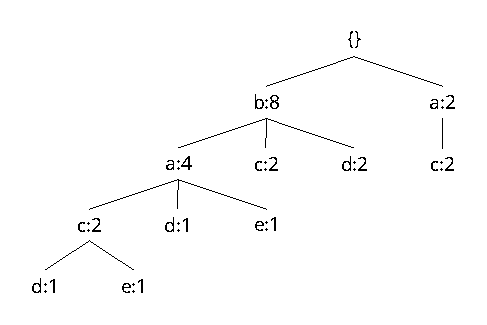
\includegraphics[width=4.5in]{problem1b.pdf}
    \end{center}
\end{figure}

\paragraph{c)}

The conditional pattern base for \(d\) is \(\{bac:1, ba:1, b:2\}\). We can see that only \(b\) and \(a\) are
frequent here, so the conditional FP-tree is the one shown below.
\begin{figure}[H]
    \begin{center}
        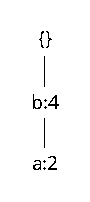
\includegraphics[width=1in]{problem1c.pdf}
    \end{center}
\end{figure}

\paragraph{d)}

Based on the conditional FP-tree we have the frequent patterns \(\{bad:2, ad:2, bd:4, d:4\}\).

\section*{Problem 2}

\paragraph{a)}

The results of my code were as follows.
\tiny
\begin{verbatim}
================================================== toy.txt
min_support: 0.6 min_conf: 0.8
Running ...

------------------------ FREQUENT PATTERNS
Itemset: "xxx", "zzz" , 60.00%
Itemset: "yyy", "zzz" , 60.00%
Itemset: "xxx", "yyy", "zzz" , 60.00%
Itemset: "xxx", "yyy" , 80.00%
----> 4 printed

------------------------ RULES:
Rule: "xxx" ==> "yyy" , 0.800
Rule: "yyy" ==> "xxx" , 1.000
Rule: "zzz" ==> "xxx" , 1.000
Rule: "zzz" ==> "yyy" , 1.000
Rule: "zzz" ==> "xxx", "yyy" , 1.000
Rule: "xxx", "zzz" ==> "yyy" , 1.000
Rule: "yyy", "zzz" ==> "xxx" , 1.000
----> 7 printed

0.00400018692017 sec


================================================== user_movies.txt
min_support: 0.26 min_conf: 0.68
Running ...

------------------------ FREQUENT PATTERNS
Itemset: "Forrest Gump (1994)", "Braveheart (1995)" , 27.33%
Itemset: "Forrest Gump (1994)", "Shawshank Redemption, The (1994)" , 28.35%
Itemset: "Pulp Fiction (1994)", "Braveheart (1995)" , 28.57%
Itemset: "Star Wars: Episode IV - A New Hope (1977)", "Star Wars: Episode V - The Empire Strikes Back (1980)" , 28.57%
Itemset: "Pulp Fiction (1994)", "Forrest Gump (1994)" , 30.10%
Itemset: "Pulp Fiction (1994)", "Shawshank Redemption, The (1994)" , 31.63%
----> 6 printed

------------------------ RULES:
Rule: "Braveheart (1995)" ==> "Forrest Gump (1994)" , 0.686
Rule: "Forrest Gump (1994)" ==> "Pulp Fiction (1994)" , 0.686
Rule: "Braveheart (1995)" ==> "Pulp Fiction (1994)" , 0.717
Rule: "Shawshank Redemption, The (1994)" ==> "Pulp Fiction (1994)" , 0.725
Rule: "Star Wars: Episode V - The Empire Strikes Back (1980)" ==> "Star Wars: Episode IV - A New Hope (1977)" , 0.897
----> 5 printed

1.05999994278 sec


================================================== movie_tags.txt
min_support: 0.0028 min_conf: 0.6
Running ...

------------------------ FREQUENT PATTERNS
Itemset: "dark comedy", "black comedy" , 0.28%
Itemset: "funny", "quirky" , 0.28%
Itemset: "future", "sci-fi" , 0.28%
Itemset: "fantasy", "adventure" , 0.29%
Itemset: "comic book", "superhero" , 0.30%
Itemset: "atmospheric", "based on a book" , 0.31%
Itemset: "Nudity (Topless)", "nudity (topless)" , 0.33%
Itemset: "sci-fi", "space" , 0.34%
Itemset: "dystopia", "sci-fi" , 0.37%
Itemset: "imdb top 250", "atmospheric" , 0.37%
Itemset: "aliens", "sci-fi" , 0.38%
Itemset: "imdb top 250", "classic" , 0.39%
Itemset: "action", "sci-fi" , 0.39%
Itemset: "stylized", "atmospheric" , 0.47%
Itemset: "funny", "comedy" , 0.57%
Itemset: "based on a book", "adapted from:book" , 0.60%
----> 16 printed

------------------------ RULES:
Rule: "future" ==> "sci-fi" , 0.729
----> 1 printed

33.2839999199 sec
\end{verbatim}
\normalsize

\paragraph{b)}

Assume for contradiction that a global frequent pattern is not a frequent pattern
of any local dataset. Let the minimum support level be \(p\). Then this implies that the pattern
appears less than \(p\) percent of the time in each local dataset, but appears more than \(p\)
percent of the time in the whole dataset. If each local dataset has less than \(p\) percent
occurrences of the pattern, then the pattern should appears less than \(p\) percent of the time in the whole
dataset. This is a contradiction, and so a global frequent pattern must be a frequent pattern
in at least one local dataset.

\paragraph{c)}

A local frequent pattern is not guaranteed to be a global frequent pattern because the local dataset
does not reflect the global dataset. For example if a local dataset had one element \(x\) and the global
dataset has one element \(x\) and 99 elements \(y\), we would find that the support of \(x\) in the
local dataset is \(100\%\) while in the global dataset it is only \(1\%\).

\section*{Problem 3}

\paragraph{a)}

\begin{align*}
    &\text{confidence}(\text{Beer}\Rightarrow\text{Nuts})=P(\text{Nuts}|\text{Beer})=\frac{150}{500}=0.3\\
    &\text{confidence}(\text{Nuts}\Rightarrow\text{Beer})=P(\text{Beer}|\text{Nuts})=\frac{150}{850}=0.1765\\
    &\text{all confidence}(\text{Beer},\text{Nuts})=0.1765\\
    &\text{lift}(\text{Beer},\text{Nuts})=\frac{150\times10000}{500\times850}=3.5294\\
    &\chi^2=\frac{(150-42.5)^2}{42.5}+\frac{(700-807.5)^2}{807.5}\\
    &\qquad+\frac{(350-457.5)^2}{457.5}+\frac{(8800-8692.5)^2}{8692.5}=312.81
\end{align*}

\paragraph{b)}

Considering that the overall probability of buying nuts is \(0.085\) and the overall probability of buying beer
is \(0.05\), I would say that the confidence values indicate that buying beer increases the chance of buying nuts and vice
versa. The lift and the \(\chi^2\) statistics reveal that these two variables are correlated as well. The lift is
greater than 1, so these variables are positively correlated. The \(\chi^2\) is very high, which means that these values
are not independent. If we were to take the \(p\)-value of this using one degree of freedom, we would find that it
would be very close to zero so we would reject the null hypothesis that these two events are independent.

\section*{Problem 4}

\paragraph{a)}

This contains six elements. The length of \(s\) is eight. It contains \(2^6-1=63\) non-empty subsequences.

\paragraph{b)}

In order to perform the join step, we must look for items that match when removing the first item from one
and the last item from another. Removing the first items yields the following sequences.
\[\{\left<ce\right>,\left<(cd)\right>,\left<ce\right>,\left<(cd)\right>,\left<bd\right>,\left<bc\right>\}\]
Removing the last items yields the following sequences.
\[\{\left<(ac)\right>,\left<bc\right>,\left<bc\right>,\left<ac\right>,\left<(ab)\right>,\left<(ab)\right>\}\]
The only matching sequence is \(\left<bc\right>\), so joining the corresponding sequences yields the following
sequences.
\[\{\left<(ab)(cd)\right>,\left<(ab)ce\right>\}\]
Then in order to prune, we must check that all the subsequences of the joined sequences are in \(L_3\). For
the first sequence \(\left<b(cd)\right>\), \(\left<a(cd)\right>\), \(\left<(ab)d\right>\), and \(\left<(ab)c\right>\)
are all in \(L_3\) so it can stay. For the next sequence \(\left<ace\right>\) and \(\left<(ab)e\right>\) are not
in \(L_3\) so we can remove it. Finally we have the following set of candidate 4-sequences \(C_4\).
\[C_4=\{\left<(ab)(cd)\right>\}\]

\end{document}